%-------------------------------------------------------------------------------
% CAPITOLO 20
%-------------------------------------------------------------------------------
\chapter{Lezione 20}
\label{capitolo_20}
\textit{13/05/2026}

\section{Potenziale di Membrana}
Il potenziale d'azione nei neuroni è una variazione rapida del potenziale di membrana che si verifica in un breve lasso di tempo. Per comprendere questo fenomeno, è necessario analizzare il comportamento della membrana cellulare e dei canali ionici che la attraversano.
La membrana cellulare del neurone, come in altre cellule, è costellata di canali ionici. Un singolo neurone può possedere diversi tipi di canali ionici, ad esempio 8 o 9 tipi, e nell'intero sistema nervoso se ne possono trovare centinaia. Questi canali ionici sono proteine che attraversano la membrana e presentano le seguenti caratteristiche:

\begin{itemize}
    \item \textbf{Sono semipermeabili:} permettono il passaggio selettivo di ioni tra l'interno e l'esterno della cellula.
    \item \textbf{Sono selettivi:} ogni tipo di canale è specifico per determinati ioni (es. canali per il Calcio, canali per il Potassio\dots).
\end{itemize}

A causa di questa semipermeabilità selettiva, si crea uno squilibrio di cariche ai due lati della membrana, generando una differenza di potenziale di membrana. Gli ioni si muovono attraverso la membrana spinti da due forze principali:

\begin{itemize}
    \item \textbf{Forza di diffusione:} dovuta a gradienti di concentrazione. Se la concentrazione di uno ione è maggiore da un lato della membrana (es. interno) rispetto all'altro (es. esterno), gli ioni tenderanno a muoversi verso la regione a minore concentrazione.
    \item \textbf{Forza elettrica:} dovuta alla differenza di potenziale elettrico attraverso la membrana. Questa forza si oppone o favorisce il movimento degli ioni a seconda della loro carica e del campo elettrico.
\end{itemize}

All'equilibrio, queste due forze si bilanciano. In una situazione di solo equilibrio diffusionale, la differenza di potenziale di membrana si attesta intorno ai $50 \text{ mV}$.


\section{Pompe Ioniche}
Oltre ai meccanismi passivi di diffusione e forza elettrica, esistono proteine chiamate pompe ioniche. Queste pompe trasportano attivamente ioni contro il loro gradiente elettrochimico, mantenendo il potenziale di membrana a un valore stazionario diverso da quello di equilibrio puramente diffusionale. Questo processo richiede energia e genera una corrente ionica netta. In presenza delle pompe ioniche, la differenza di potenziale attraverso un singolo canale ionico può raggiungere valori dell'ordine di $50-100 \text{ mV}$. Il valore esatto dipende dal tipo specifico di canale ionico considerato.


\section{Modellizzazione della Membrana Come Capacitore}
La membrana cellulare, nel suo complesso, può essere schematizzata come un capacitore, poiché separa cariche elettriche sui suoi due lati. Se $C$ è la capacità dell'intera membrana e $V$ è la differenza di potenziale ai suoi capi, la variazione di potenziale nel tempo è data da:

\begin{equation} \label{eq:ch20_1}
C\frac{dV}{dt} = I_{tot}
\end{equation}

La corrente totale $I_{tot}$ può essere suddivisa in due contributi principali:
\begin{itemize}
    \item $I_{Ch}$: la corrente dovuta al passaggio di ioni attraverso i canali ionici.
    \item $I_{ext}$: una corrente esterna, ad esempio un segnale elettrico proveniente da altri neuroni connessi.
\end{itemize}

Quindi, l'equazione diventa:

\begin{equation} \label{eq:ch20_2}
C\frac{dV}{dt} = I_{Ch} + I_{EXT}
\end{equation}

La corrente attraverso i canali $I_{Ch}$ è la somma dei contributi di tutti i tipi di canali presenti. Se $n$ è il numero di diversi tipi di canali:

\begin{equation} \label{eq:ch20_3}
I_{Ch} = \sum_{i=1}^{n} N_{i}f_{i}g_{i}(V_{i}-V)
\end{equation}

Dove:
\begin{itemize}
    \item $N_i$: è il numero di canali del tipo $i$-esimo sulla membrana (una costante che rappresenta l'abbondanza di quel tipo di canale).
    \item $f_i$: è la frazione di canali del tipo $i$-esimo che sono aperti. Questa frazione dipende dal potenziale di membrana $V$.
    \item $g_i$: è la conduttanza di un singolo canale aperto del tipo $i$-esimo ($g_i = 1/R_i$, dove $R_i$ è la resistenza del canale).
    \item $V_i$: è il potenziale di riposo (o di inversione) per il canale di tipo $i$-esimo. È il valore del potenziale di membrana $V$ al quale la corrente attraverso il canale di tipo $i$ si annulla. Se $V=V_i$, non c'è flusso netto di corrente attraverso quel specifico tipo di canale, anche se potrebbe esserci corrente attraverso altri tipi di canali.
\end{itemize}

Il prodotto $g_i(V_i-V)$ rappresenta la corrente che fluisce attraverso un singolo canale aperto di tipo $i$.


\section{Dinamica della Frazione di Canali Aperti}
La frazione di canali aperti $f_i$ non è costante ma dipende essa stessa dal potenziale $V$. Questa dipendenza è cruciale perché introduce un meccanismo di feedback che permette l'apertura rapida e concertata di molti canali, alla base dell'impulso nervoso.
Si può assumere che $f_i$ tenda a un valore di equilibrio $f_i^{eq}(V)$ che dipende dal potenziale istantaneo $V$. La dinamica con cui $f_i$ si avvicina a questo valore di equilibrio può essere descritta da un'equazione di rilassamento esponenziale:

\begin{equation} \label{eq:ch20_4}
\frac{df_{i}}{dt} = -\frac{1}{\tau_{i}}[f_{i}-f_{i}^{eq}(V)]
\end{equation}

Dove $\tau_i$ è la costante di tempo caratteristica per l'apertura/chiusura dei canali di tipo $i$. Canali diversi possono avere $\tau_i$ diversi (canali rapidi o lenti).
Il sistema completo di equazioni da risolvere è quindi costituito dall'equazione per $dV/dt$ e dalle $n$ equazioni per $df_i/dt$:

\vspace{0.5cm}
\noindent\fbox{%
    \parbox{\dimexpr\linewidth-2\fboxsep-2\fboxrule\relax}{%
        \begin{equation} \label{eq:ch20_5}
        \begin{cases}  
        \frac{df_{i}}{dt} &= -\frac{1}{\tau_{i}}[f_{i}-f_{i}^{eq}(V)] \\ \\ 
        C\frac{dV}{dt} &= \sum_{i=1}^{n} N_{i}f_{i}g_{i}(V_{i}-V) + I_{EXT} 
        \end{cases} 
        \end{equation}
    }%
}
\vspace{0.5cm}


\section{Determinazione di $f_i^{eq}(V)$: Modello a Due Stati}
Per determinare $f_i^{eq}(V)$, consideriamo un singolo canale che può esistere in due stati: aperto (O) o chiuso (C).
Quando un canale si apre, una certa quantità di carica, detta gating charge $Q_{eff}$ (carica efficace, che può essere un multiplo della carica elementare $e$, cioè $Q \cdot e$), si muove attraverso la membrana, che si trova a un potenziale $V$. Questo movimento di carica comporta una variazione dell'energia libera del canale.
Siano $F_{i0}^C$ e $F_{i0}^O$ le energie libere del canale di tipo $i$ rispettivamente nello stato chiuso e aperto, in assenza dell'effetto del potenziale di membrana sulla gating charge.

Quando il potenziale di membrana è $V$:
\begin{itemize}
    \item Energia libera dello stato chiuso: $E_C = F_{i0}^C$
    \item Energia libera dello stato aperto: $E_O = F_{i0}^O - Q_{eff}V$
\end{itemize}

Il termine $-Q_{eff}V$ rappresenta la diminuzione di energia dovuta al movimento della gating charge $Q_{eff}$ secondo il potenziale $V$.
Utilizzando la statistica di Boltzmann, la probabilità che il canale sia aperto, $P_i^O$, che corrisponde a $f_i^{eq}(V)$, è data da:

\begin{equation} \label{eq:ch20_6}
P_i^O = \frac{e^{-\beta E_O}}{e^{-\beta E_O} + e^{-\beta E_C}} = \frac{e^{-\beta (F_{i0}^O - Q_{eff}V)}}{e^{-\beta (F_{i0}^O - Q_{eff}V)} + e^{-\beta F_{i0}^C}}
\end{equation}

Questa espressione può essere riscritta dividendo numeratore e denominatore per $e^{-\beta (F_{i0}^O - Q_{eff}V)}$:

\begin{equation} \label{eq:ch20_7}
P_i^O  = \frac{1}{1 + e^{\beta [F_{i0}^O - F_{i0}^C - Q_{eff}V]}}
\end{equation}

Questa è una funzione sigmoidale e può essere espressa nella forma standard:

\vspace{0.5cm}
\noindent\fbox{%
    \parbox{\dimexpr\linewidth-2\fboxsep-2\fboxrule\relax}{%
        \begin{equation} \label{eq:ch20_8}
        f_i^{eq}(V) = P_i^O(V) = \frac{1}{1+e^{-\frac{(V-V_{1/2,i})}{\Delta_i}}}
        \end{equation}
    }%
}
\vspace{0.5cm}

Dove:
\begin{itemize}
    \item $V_{1/2,i} = \frac{F_{i0}^C - F_{i0}^O}{Q_{eff}}$ è il potenziale al quale metà dei canali di tipo $i$ sono aperti ($f_i^{eq}(V_{1/2,i}) = 1/2$).
    \item $\Delta_i = \frac{1}{Q_{eff}\beta}$ è un parametro che determina la pendenza della curva sigmoidale, rappresentando una scala di potenziale per la sensibilità del canale.
\end{itemize}

La funzione $f_i^{eq}(V)$ è quindi non lineare, il che rende il sistema di equazioni differenziali accoppiate difficile da risolvere analiticamente in generale.

\begin{figure}[h!]
\centering
% 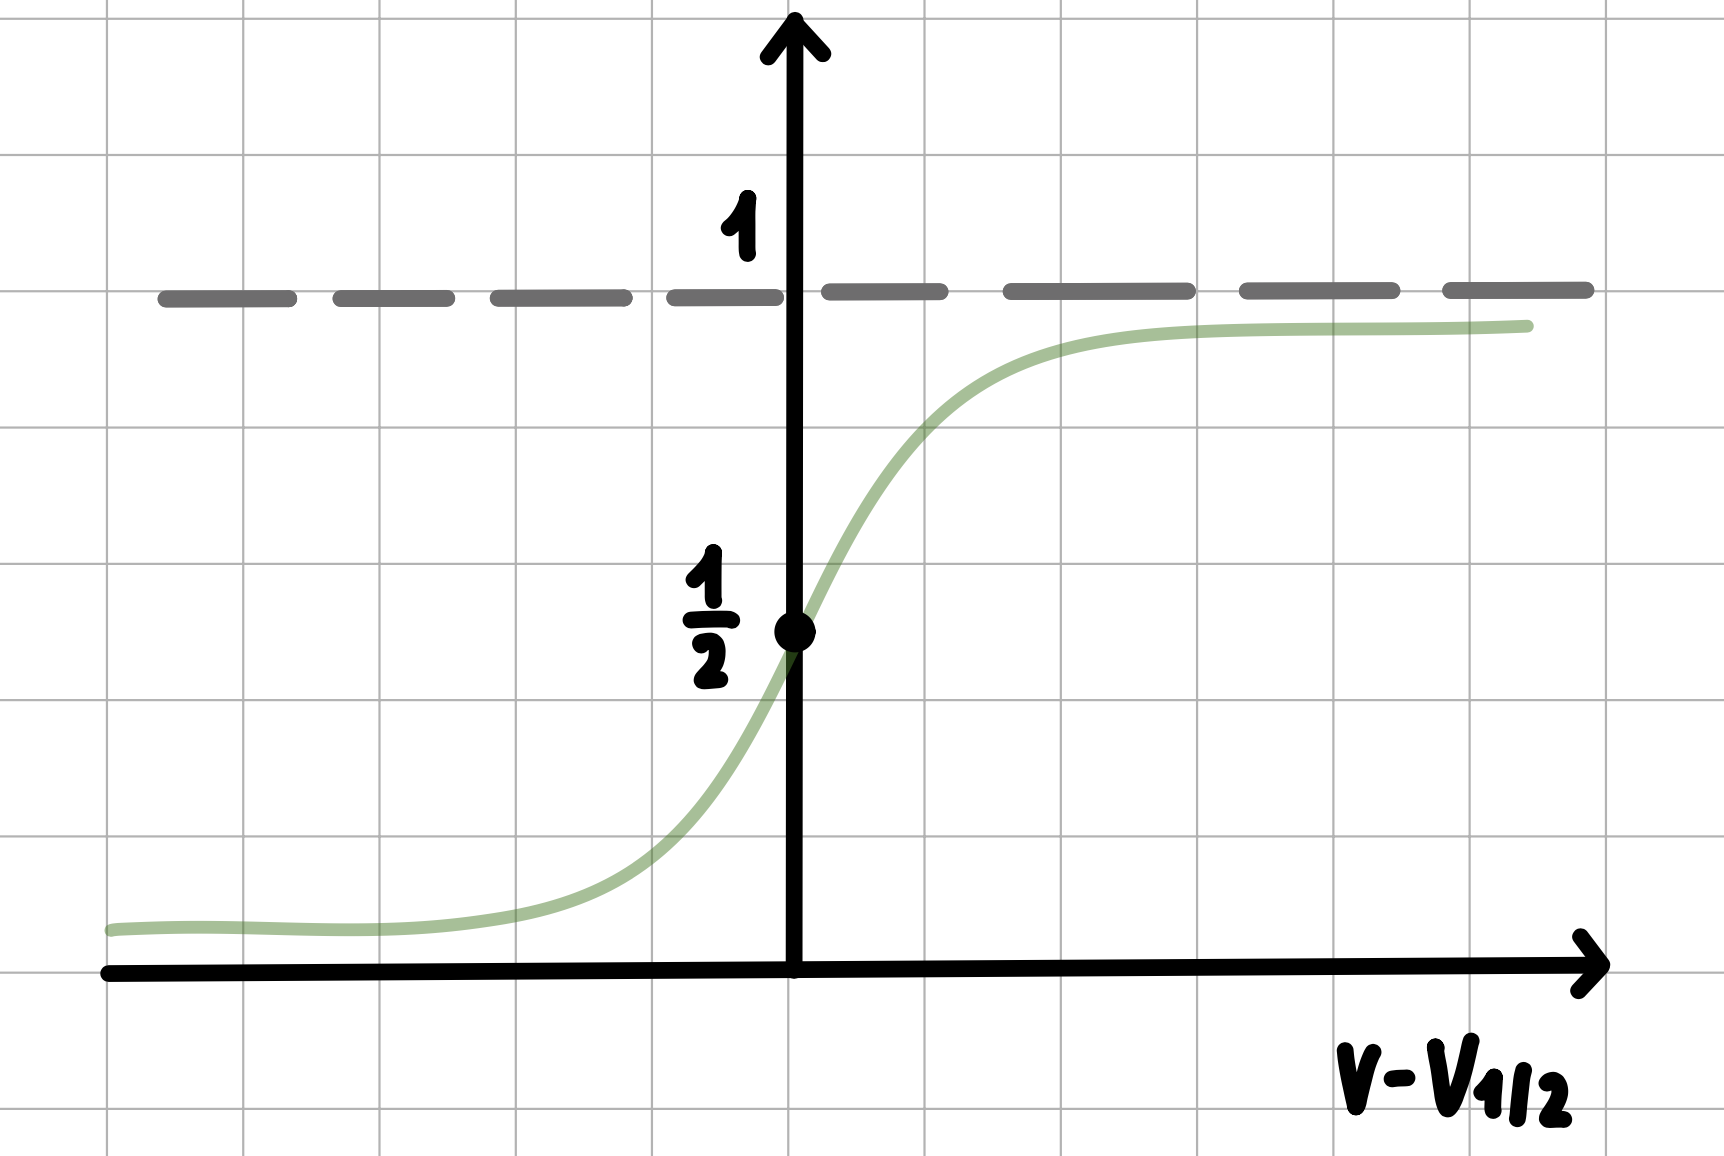
\includegraphics[width=0.6\textwidth]{pics/20_1.png} % INSERIRE QUI IL GRAFICO DELLA FUNZIONE SIGMOIDE
\caption{Curva sigmoidale che descrive la frazione di canali aperti all'equilibrio $f_i^{eq}(V)$ in funzione del potenziale di membrana $V$.}
\label{fig:ch20_1}
\end{figure}


\section{Linearizzazione del Sistema}
Per analizzare il comportamento del sistema, si può ricorrere a una linearizzazione attorno a uno stato stazionario. Assumiamo che il sistema si trovi inizialmente in uno stato stazionario $V_0$ (in assenza di segnali esterni, $\delta I_{EXT}=0$). Applichiamo una piccola perturbazione $\delta I_{EXT}$ che causa piccole variazioni $\delta V$ e $\delta f_i$:

\begin{equation} \label{eq:ch20_9}
\begin{cases}
V(t) &= V_0 + \delta V(t) \\ 
f_i(t) &= f_{i0} + \delta f_i(t) \\ 
f_{i0} &= f_i^{eq}(V_0) 
\end{cases}
\end{equation}

Espandiamo $f_i^{eq}(V)$ attorno a $V_0$:

\begin{equation} \label{eq:ch20_10}
f_i^{eq}(V_0 + \delta V) \approx f_i^{eq}(V_0) + \left.\frac{\partial f_i^{eq}}{\partial V}\right|_{V_0} \delta V 
\end{equation}

Sostituiamo nelle equazioni originali (\ref{eq:ch20_5}):

Per $dV/dt$, si parte da:

\begin{equation} \label{eq:ch20_11}
C\frac{d\delta V}{dt} = \sum_{i=1}^{n}N_{i}g_{i}(f_{i0}+\delta f_{i})[V_{i}-(V_{0}+\delta V)]+I_{EXT}
\end{equation}

Espandendo i prodotti:

\begin{equation*}
C\frac{d\delta V}{dt} = \sum_{i=1}^{n}N_{i}g_{i}(f_{i0}(V_i-V_{0}) - f_{i0}\delta V + \delta f_{i}(V_i-V_{0}) - \delta f_{i}\delta V) + I_{EXT}
\end{equation*}

Nello stato stazionario $V_0$, in assenza di perturbazione esterna ($I_{EXT,0}=0$), si ha:

\begin{equation} \label{eq:ch20_12}
0 = \sum_{i}N_{i}g_{i}f_{i0}(V_{i}-V_{0})
\end{equation}

Trascurando i termini del secondo ordine (come $\delta f_i \delta V$), l'equazione linearizzata per $\delta V$ (con $\delta I$ indicante la perturbazione $I_{EXT}$) è:

\begin{equation} \label{eq:ch20_13}
C\frac{d\delta V}{dt} = \sum_{i=1}^{n}N_{i}g_{i}[-f_{i}^{eq}(V_{0})\delta V + (V_{i}-V_{0})\delta f_{i}] + \delta I
\end{equation}

Per $df_i/dt$, si parte da:

\begin{equation} \label{eq:ch20_14}
\frac{d\delta f_{i}}{dt} = -\frac{1}{\tau_{i}}\Bigg[(f_{i0}+\delta f_{i})-\left(f_{i}^{eq}(V_{0})+\left.\frac{\partial f_{i}^{eq}}{\partial V}\right|_{V_{0}}\delta V\right)\Bigg]
\end{equation}

Che si semplifica a:

\begin{equation} \label{eq:ch20_15}
\frac{d\delta f_{i}}{dt} = -\frac{1}{\tau_{i}}\left[\delta f_{i} - \left.\frac{\partial f_{i}^{eq}}{\partial V}\right|_{V_{0}}\delta V\right]
\end{equation}


\section{Analisi nel Dominio di Fourier}
Per risolvere questo sistema di equazioni differenziali lineari, passiamo al dominio di Fourier.
Definiamo la trasformata di Fourier di una funzione $x(t)$ come:
$\hat{x}(\omega) = \int x(t)e^{i\omega t}dt$
La derivata $dx/dt$ si trasforma in $-i\omega \hat{x}(\omega)$

Le equazioni linearizzate trasformate diventano:

\begin{equation} \label{eq:ch20_16}
-i\omega C \delta\hat{V}(\omega) = -\sum_{i}N_ig_{i}f_{i0}\delta\hat{V}(\omega) + \sum_{i}N_ig_{i}(V_{i}-V_{0})\delta\hat{f}_{i}(\omega) + \delta\hat{I}(\omega)
\end{equation}

\begin{equation} \label{eq:ch20_17}
-i\omega\delta\hat{f}_{i}(\omega) = -\frac{1}{\tau_{i}}\left[\delta\hat{f}_{i}(\omega) - \left.\frac{df_{i}^{eq}}{dV}\right|_{V_{0}}\delta\hat{V}(\omega)\right]
\end{equation}

Dalla seconda equazione, possiamo esprimere $\delta\hat{f}_{i}(\omega)$ in termini di $\delta\hat{V}(\omega)$:

\begin{equation} \label{eq:ch20_18}
\delta\hat{f}_{i}(\omega) = \frac{1}{1-i\omega\tau_{i}}\left.\frac{df_{i}^{eq}}{dV}\right|_{V_{0}}\delta\hat{V}(\omega)
\end{equation}

Sostituendo questa espressione nella (\ref{eq:ch20_16}):

\begin{align*} 
-i\omega C \delta\hat{V}(\omega) &= -\left(\sum_{i}N_ig_{i}f_{i0}\right)\delta\hat{V}(\omega) \\
&+ \sum_{i}N_ig_{i}(V_{i}-V_{0})\frac{1}{1-i\omega\tau_{i}}\left.\frac{df_{i}^{eq}}{dV}\right|_{V_{0}}\delta\hat{V}(\omega)\\ 
&+ \delta\hat{I}(\omega) 
\end{align*}

Raccogliendo i termini con $\delta\hat{V}(\omega)$:

\begin{align} \label{eq:ch20_19}
\delta\hat{I}(\omega) = \delta\hat{V}(\omega) \left\{ -i\omega C + \sum_{i}N_ig_{i} \Bigg[ f_{i0} - \frac{(V_{i}-V_{0})}{1-i\omega\tau_{i}}\left.\frac{df_{i}^{eq}}{dV}\right|_{V_{0}} \Bigg]\right\} 
\end{align}

Definendo la conduttanza di base $1/R_0 = \sum_{i}N_ig_{i}f_{i0}$ (la conduttanza totale della membrana nello stato stazionario $V_0$ dovuta alla frazione basale di canali aperti):

\vspace{0.5cm}
\noindent\fbox{%
    \parbox{\dimexpr\linewidth-2\fboxsep-2\fboxrule\relax}{%
        \begin{equation} \label{eq:ch20_20}
        \delta\hat{I}(\omega) = \delta\hat{V}(\omega) \left\{ -i\omega C + \frac{1}{R_{0}} + \sum_{i}N_ig_{i}\frac{(V_{0}-V_{i})}{1-i\omega\tau_{i}}\left.\frac{df_{i}^{eq}}{dV}\right|_{V_{0}} \right\}
        \end{equation}
    }%
}
\vspace{0.5cm}

Questa equazione lega la perturbazione di corrente applicata $\delta\hat{I}(\omega)$ alla risposta in potenziale $\delta\hat{V}(\omega)$ attraverso un'impedenza generalizzata $Z(\omega)$, dove $\delta\hat{V}(\omega) = Z(\omega)\delta\hat{I}(\omega)$.
L'espressione tra parentesi graffe è l'ammettenza $Y(\omega) = 1/Z(\omega)$.


\section{Analisi dei Casi Limite del Termine di Somma}
Il termine $\sum_{i}N_ig_{i}\frac{(V_{0}-V_{i})}{1-i\omega\tau_{i}}\left.\frac{df_{i}^{eq}}{dV}\right|_{V_{0}}$ modifica l'ammettenza del sistema in modo dipendente dalla frequenza.

\subsection*{Canali Veloci ($\tau_i \omega \ll 1$)}
Per canali con costante di tempo $\tau_i$ molto piccola, il termine $1-i\omega\tau_i \approx 1$.
Il contributo all'ammettenza diventa una conduttanza costante:

\begin{equation} \label{eq:ch20_21}
\sum_{i \in \text{veloci}} N_ig_{i}(V_{0}-V_{i})\left.\frac{df_{i}^{eq}}{dV}\right|_{V_{0}}
\end{equation}

Consideriamo le condizioni per un feedback positivo:
\begin{itemize}
    \item $\left.\frac{df_{i}^{eq}}{dV}\right|_{V_{0}} > 0$: un aumento di $V$ apre più canali (sensibilità positiva).
    \item $V_i > V_0$: il potenziale di inversione del canale è maggiore del potenziale di riposo $V_0$. Questo implica che allo stato $V_0$ c'è una forza spingente per l'ingresso di cariche positive (o uscita di negative) se il canale si apre.
\end{itemize}

In queste condizioni, il termine $(V_0 - V_i)$ è negativo. Quindi, il contributo di questi canali alla conduttanza $(V_0-V_i) \cdot (df/dV)$ è \textbf{negativo}. Una conduttanza negativa effettiva riduce la resistenza totale del circuito, potenziando la risposta a una perturbazione (feedback positivo).

\subsection*{Canali Lenti ($\tau_i \omega \gg 1$)}
Per canali con costante di tempo $\tau_i$ molto grande, il termine $1-i\omega\tau_i \approx -i\omega\tau_i$.
Il contributo all'ammettenza diventa:

\begin{equation} \label{eq:ch20_22}
\sum_{i \in \text{lenti}} N_ig_{i}(V_{0}-V_{i})\left.\frac{df_{i}^{eq}}{dV}\right|_{V_{0}} \frac{1}{-i\omega\tau_i} = \frac{1}{i\omega} \sum_{i \in \text{lenti}} N_ig_{i}\frac{(V_{i}-V_{0})}{\tau_{i}}\left.\frac{df_{i}^{eq}}{dV}\right|_{V_{0}}
\end{equation}

Questo termine ha la forma $1/(i\omega L_{eff})$, che è l'ammettenza di un'induttanza efficace $L_{eff}$, dove:

\begin{equation} \label{eq:ch20_23}
L_{eff} = \left( \sum_{i \in \text{lenti}} N_ig_{i}\frac{(V_{i}-V_{0})}{\tau_{i}}\left.\frac{df_{i}^{eq}}{dV}\right|_{V_{0}} \right)^{-1}
\end{equation}

Quindi, i canali lenti possono conferire proprietà \textbf{induttive} alla membrana neuronale a certe frequenze.

Questi comportamenti (conduttanza negativa per canali veloci, induttanza per canali lenti) sono importanti per determinare la risposta dinamica del neurone a segnali variabili nel tempo e possono contribuire a fenomeni come la risonanza e l'eccitabilità neuronale.
